\documentclass[11pt]{article}

\usepackage[a4paper,margin=25mm,headheight=15pt]{geometry}
\usepackage[T1]{fontenc}
\usepackage[utf8]{inputenc}
\usepackage{lmodern}
\usepackage{microtype}
\usepackage{amsmath}
\usepackage{booktabs}
\usepackage{array}
\usepackage{longtable}
\usepackage{enumitem}
\usepackage{xcolor}
\usepackage{fancyhdr}
\usepackage{tikz}
\usetikzlibrary{arrows.meta,positioning,shapes.geometric}
\usepackage[hidelinks]{hyperref}
\usepackage{xr}
% Cross-references to the separate Supplementary Figures document (S1-S11).
% Compile supplementary_figures.tex first so its .aux is available.
\externaldocument{supplementary_figures}

\definecolor{Accent}{HTML}{315B7D}
\definecolor{NoteBlue}{HTML}{EAF2F8}
\definecolor{NoteBorder}{HTML}{7BA5C4}
\definecolor{Muted}{HTML}{5B6570}

\hypersetup{
  pdftitle={Materials and Methods: LD decay, complexity reduction, ancestry sorting, genomic architecture, and climate association},
  pdfauthor={Poikela et al.},
  pdfsubject={Hybrid genome evolution in Formica wood ants}
}

\pagestyle{fancy}
\fancyhf{}
\lhead{\small\color{Muted}Materials and Methods}
\rhead{\small\color{Muted}Poikela et al.}
\cfoot{\small\thepage}
\renewcommand{\headrulewidth}{0.4pt}

\setlength{\parindent}{0pt}
\setlength{\parskip}{0.65em}
\setlist[itemize]{leftmargin=1.5em,itemsep=0.2em,topsep=0.25em}
\setlist[enumerate]{leftmargin=1.7em,itemsep=0.25em,topsep=0.25em}
\renewcommand{\arraystretch}{1.15}
\renewcommand{\thesection}{S\arabic{section}}
\renewcommand{\thesubsection}{\thesection.\arabic{subsection}}

\newcommand{\Faq}{\textit{F.~aquilonia}}
\newcommand{\Fpo}{\textit{F.~polyctena}}
\newcommand{\rsq}{\ensuremath{r^{2}}}
\newcommand{\todo}[1]{%
  \par\noindent
  \fcolorbox{NoteBorder}{NoteBlue}{%
    \parbox{\dimexpr\linewidth-2\fboxsep-2\fboxrule\relax}{%
      \textbf{Open item.} #1}}%
  \par}
\newcommand{\couldstill}[1]{%
  \par\noindent
  \fcolorbox{NoteBorder}{NoteBlue}{%
    \parbox{\dimexpr\linewidth-2\fboxsep-2\fboxrule\relax}{%
      \textbf{Could still be done.} #1}}%
  \par}

\title{\vspace{-3em}
  \textbf{\color{Accent}Materials and Methods}\\[0.3em]
  \Large LD decay, LD-based complexity reduction, and analyses of ancestry
  sorting, genomic architecture, and climate association}
\author{Poikela et al.}
\date{\small Draft prepared from the current \texttt{/doc} pipeline documentation}

\begin{document}
\maketitle
\vspace{-1.5em}

\begin{center}
\small\color{Muted}
This is a self-contained working draft for integration into the full
Supplementary Materials. Blue boxes identify editorial or computational items
that remain open and are not intended as final manuscript text.
\end{center}

\section{Scope and analytical principles}

These methods describe LD decay estimation, LD-based complexity reduction,
quantification of the extent and direction of ancestry sorting, analysis of its
genomic architecture, and tests of whether ancestry-diagnostic or directionally
sorted loci occur preferentially in regions whose allele frequencies covary
with climate.

Three principles guided the analyses. First, markers in LD carry partly
redundant information. We therefore used clusters of strongly correlated
markers as LD-reduced analytical units wherever possible, while retaining
marker-level analyses as diagnostics of spatial pseudoreplication. We do not
assume that the resulting units are strictly statistically independent.
Second, a variable evaluated as a predictor was not also used to select the
analysed data. In particular, loci were gated by parental allele frequency
rather than by the diagnostic index (DI), leaving the full range of DI
available for analysis. Third, cluster-level criteria were expressed as rates
rather than fixed counts when a count would make eligibility depend
non-linearly on cluster size.

The twenty hybrid populations provide repeated observations of ancestry
sorting across geographically separated populations. However, their
evolutionary histories need not be fully independent. We therefore refer to
them as replicate or sampled hybrid populations without assuming independent
origins or complete demographic independence. Analyses that use variation
among populations either model their covariance explicitly or are interpreted
as descriptive associations.

\begin{figure}[p]
\centering
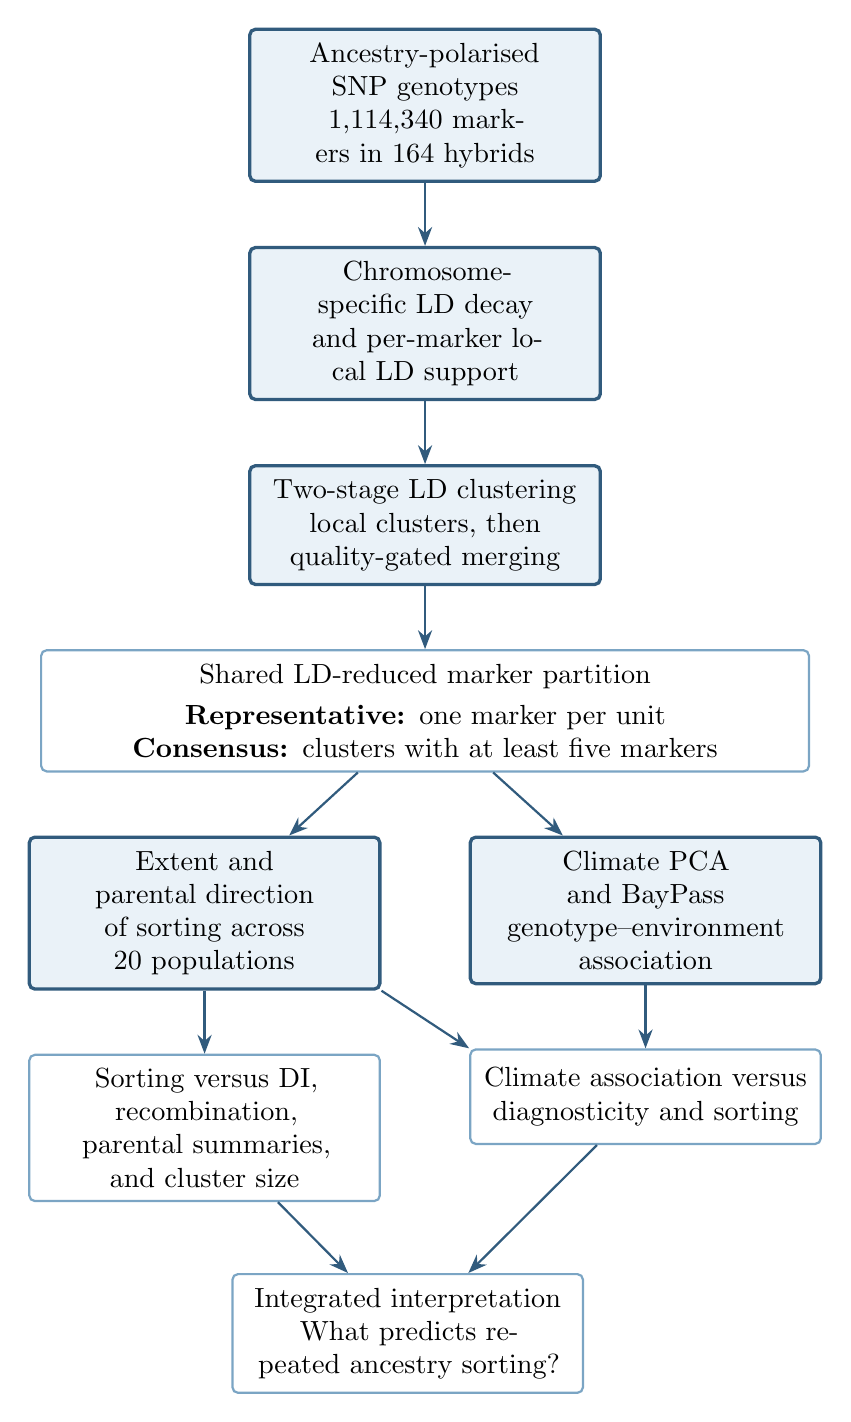
\begin{tikzpicture}[
  node distance=8mm and 12mm,
  box/.style={
    draw=Accent, rounded corners=2pt, very thick, fill=NoteBlue,
    align=center, text width=41mm, minimum height=12mm, inner sep=5pt
  },
  result/.style={
    draw=NoteBorder, rounded corners=2pt, thick, fill=white,
    align=center, text width=41mm, minimum height=12mm, inner sep=5pt
  },
  arrow/.style={-{Stealth[length=2.4mm]}, thick, draw=Accent}
]
\node[box] (genotypes) {Ancestry-polarised SNP genotypes\\
1,114,340 markers in 164 hybrids};
\node[box, below=of genotypes] (ld) {Chromosome-specific LD decay\\
and per-marker local LD support};
\node[box, below=of ld] (cluster) {Two-stage LD clustering\\
local clusters, then quality-gated merging};
\node[result, below=of cluster, text width=94mm] (projections)
{Shared LD-reduced marker partition\\[1mm]
\textbf{Representative:} one marker per unit\\
\textbf{Consensus:} clusters with at least five markers};
\node[box, below=of projections, xshift=-28mm] (sorting)
{Extent and parental direction\\
of sorting across 20 populations};
\node[box, below=of projections, xshift=28mm] (climate)
{Climate PCA and BayPass\\
genotype--environment association};
\node[result, below=of sorting] (architecture) {Sorting versus DI,\\
recombination, parental summaries,\\
and cluster size};
\node[result, below=of climate] (overlap) {Climate association versus\\
diagnosticity and sorting};
\node[result, below right=9mm and -19mm of architecture] (synthesis)
{Integrated interpretation\\
What predicts repeated ancestry sorting?};

\draw[arrow] (genotypes) -- (ld);
\draw[arrow] (ld) -- (cluster);
\draw[arrow] (cluster) -- (projections);
\draw[arrow] (projections) -- (sorting);
\draw[arrow] (projections) -- (climate);
\draw[arrow] (sorting) -- (architecture);
\draw[arrow] (climate) -- (overlap);
\draw[arrow] (sorting.south east) -- (overlap.north west);
\draw[arrow] (architecture) -- (synthesis);
\draw[arrow] (overlap) -- (synthesis);
\end{tikzpicture}
\caption{\textbf{Analytical workflow.} LD decay and clustering transform the
marker data into a shared set of LD-reduced units represented either by a
single marker or, for larger clusters, by a consensus genotype. The same units
then connect the analyses of ancestry sorting, genomic architecture, and
climate association.}
\label{fig:workflow}
\end{figure}
\clearpage

\section{Samples, genotypes, and ancestry polarisation}

\subsection{Samples}

The analysis included twenty \Faq{} $\times$ \Fpo{} hybrid populations sampled
from nineteen locations in Finland and one location in Switzerland, together
with allopatric reference samples of the parental species. The current analysis
objects contain 164 diploid hybrid individuals. The analyses described here
concern this diploid hybrid data set.

\todo{The general sample description currently reports 165 sequenced hybrid
individuals, whereas the analysis objects contain 164. Confirm which individual
was excluded, most likely because of excessive missing data, and report the
identifier and exclusion criterion in the final text. Until then, 164 is used
for all analysis-specific counts.}

\subsection{Marker processing and ancestry orientation}

Genotypes and marker-level ancestry information were obtained from the DIEM
output for this data set. Sites were restricted to biallelic markers. DIEM
provides a polarity and a diagnostic index for each marker. The diagnostic
index measures the degree to which allele frequencies differentiate the
parental reference samples. For markers with the opposite polarity, genotype
dosages were replaced by \(2-\mathrm{dosage}\), placing dosages on a consistent
ancestry-oriented scale across the genome.

Minor allele frequency (MAF) was calculated among hybrid individuals only, and
markers with hybrid MAF \(\geq 0.05\) were retained. The resulting analysis set
contained 1,114,340 markers. Two matrices were constructed over this same
marker set. The hybrids-only matrix was used for LD estimation, clustering, and
complexity reduction. A second matrix containing hybrids and parental
references was used when parental allele frequencies were required, including
ancestry orientation and marker-level parental summaries. Keeping the parents
out of the LD calculations prevents
parent--hybrid differentiation from dominating estimates intended to describe
LD within the hybrid populations.

\section{LD decay and local LD support}

\subsection{Chromosome-specific LD decay}

LD decay was modelled separately for each chromosome as
\begin{equation}
  r^2(d) = b + \frac{c-b}{1+a d},
  \label{eq:lddecay}
\end{equation}
where \(d\) is physical distance in base pairs, \(a\) is the decay rate,
\(b\) is long-range background \(r^2\), and \(c\) is short-range \(r^2\).
Background LD was estimated from inter-chromosomal marker pairs. Within each
chromosome, the curve was fitted across twenty sliding windows with 50\%
overlap. Up to 5,000 marker pairs were sampled per window, stratified across
twenty distance classes to represent short and long distances comparably. The
0.95 quantile of \(r^2\) was used as the within-class summary, and parameter
estimates were aggregated over the central 95\% of windows to reduce the
influence of outlying fits (Fig.~\ref{figS:lddecay}).

Only pairs for which both markers had MAF \(>0.1\) contributed to the
background and decay-curve fits. This restriction reduces the frequency-driven
depression of \(r^2\) at rare alleles. It was applied only during curve fitting;
the stored LD edge lists retained the complete marker set used for clustering.

Decay rate varied with chromosome length. A robust regression of \(a\) on
chromosome size was therefore fitted genome-wide. For a relative LD threshold
\(\rho\), the corresponding physical distance was calculated as
\begin{equation}
  d = \frac{\rho}{a(1-\rho)}.
  \label{eq:distance}
\end{equation}
This allowed window sizes to reflect each chromosome's fitted decay behaviour
rather than imposing one physical-distance threshold across the genome.

\subsection{Per-marker local LD support}

For each marker, local LD support (\(\mathrm{ld}_w\)) was calculated as the
median \(r^2\) between that marker and neighbouring markers within the window
corresponding to \(\rho=0.95\). Unlike map-based recombination rate,
\(\mathrm{ld}_w\) is measured directly from the genotype data at marker
resolution and requires no interpolation.

We evaluated \(\mathrm{ld}_w\) and the window-level decay rate \(a\) as
indicators of low recombination using map-based recombination rate as a
reference. Across definitions based on the lowest 5\%, 10\%, and 25\% of
recombination windows, the area under the receiver-operating-characteristic
curve was 0.91--0.98 for \(a\) and 0.73--0.86 for \(\mathrm{ld}_w\).
Accordingly, \(a\) was the stronger window-level indicator, whereas
\(\mathrm{ld}_w\) supplied the marker-resolution measure needed to identify
clusters for reconsideration during complexity reduction
(Figs~\ref{figS:roc} and~\ref{figS:tracks}).

\section{Two-stage LD-based complexity reduction}

\subsection{Terminology and outputs}

The procedure has two stages: (1) local clustering with a complete-linkage
refinement and (2) targeted, quality-gated merging. Both stages define a single
partition of markers, from which two representations are produced:
\begin{itemize}
  \item one representative marker per cluster, forming an LD-pruned marker set;
  \item one expected multi-locus genotype (eMLG) consensus dosage for clusters
        containing at least five markers.
\end{itemize}

We use ``LD cluster'' or ``LD-reduced unit'' for a set of strongly correlated
markers. These units are not haplotype blocks: markers are grouped by the
partition of sampled chromosomes that they report, and clusters may therefore
overlap in physical position. Nor do we describe them as strictly independent.
The procedure reduces redundancy and constrains residual LD; the remaining
dependence is assessed or controlled where it matters downstream.

\subsection{Stage 1: local clustering}

For each chromosome, the clustering distance was derived from its fitted LD
decay curve at \(\rho=0.5\). The threshold was not allowed to vary further
within chromosomes, because locally elevated LD is precisely where redundant
markers should be grouped more strongly.

Clustering was performed on the precomputed sparse LD graph. Markers were first
assigned to connected components of the thresholded graph. Each component was
then refined by complete-linkage hierarchical clustering using the dense
pairwise \(r^2\) matrix within the component. The complete-linkage step limits
single-linkage chaining, in which two weakly correlated markers could otherwise
be joined through an intermediate marker correlated with both.

The representative marker of a cluster was the member with the highest median
\(r^2\) to the other cluster members.

\subsection{Stage 2: targeted, quality-gated merging}

The finite window used to construct the Stage 1 edge list makes the first stage
conservative in extended low-recombination regions: marker pairs outside the
window are not evaluated and therefore cannot satisfy complete linkage. Stage
2 reconsidered candidate clusters directly from their genotypes, without the
Stage 1 window restriction.

A Stage 1 cluster was flagged if any member had
\(\mathrm{ld}_w>0.025\), or if the cluster contained at least five markers.
Flagged clusters were considered for merging using a distance-restricted,
average-linkage dynamic tree cut. A candidate merge was accepted only while
both of the following criteria were satisfied:
\begin{enumerate}
  \item consensus fidelity
  \[
    \mathrm{score}_{\mathrm{eMLG}}(x)
    =\mathrm{cor}\{\mathrm{round}(x),x\}^{2} \geq 0.80;
  \]
  \item a pairwise correlation floor of \(r^2\geq0.2\) between the sides being
        merged.
\end{enumerate}

The fidelity criterion evaluates whether the resulting consensus remains close
to a discrete genotype. The correlation floor prevents a small, weakly related
set of markers from being absorbed into a large cluster whose existing
consensus would otherwise dominate the fidelity score. These gates constrain
merging but do not establish complete statistical independence among the final
units. Observed residual correlations among neighbouring merged units were of
order \(r^2\approx0.3\) after correction for relatedness and were local in
genetic distance.

Candidate merges were restricted to 0.5 cM using the genetic map. Genetic rather
than physical distance was used because a common physical distance represents
different recombination distances across chromosomes and genomic regions.

\subsection{Output and validation}

The final partition contained 474,014 LD clusters. Of these, 32,840 contained
at least five markers and had an eMLG consensus. Smaller
clusters remain valid LD-reduced units and retain their representative marker;
the five-marker threshold is therefore a threshold for storing a consensus,
not for defining a cluster.

The procedure was evaluated by comparing Stage 1 and combined Stage 1--2
clusterings in extended-LD regions (Fig.~\ref{figS:stage}), by examining the
distribution of consensus fidelity across \(\mathrm{ld}_w\) thresholds
(Fig.~\ref{figS:fidelity}), and by quantifying the ability of
\(\mathrm{ld}_w\) to identify low-recombination regions. These checks assess
whether Stage 2 consolidates fragmentation where long-range LD is present
without broadly collapsing weakly correlated markers.

\section{Extent and direction of ancestry sorting}

\subsection{Near-fixation and ancestry orientation}

For each marker or cluster consensus, dosage was oriented as the
\Faq-allele frequency using the sign of the parental allele-frequency
difference. Units for which the parents did not differ had no defined parental
direction. Within each hybrid population, a unit was classified as near-fixed
toward \Faq{} when the oriented allele frequency was at least
\(1-\theta\), near-fixed toward \Fpo{} when it was at most \(\theta\), and
otherwise not near-fixed, with \(\theta=0.15\). The same tolerance was used
throughout because the attainable frequency values depend on the number of
sampled diploid individuals in a population.

\subsection{Sorting decomposition and classification}

Let \(n_{\mathrm{obs}}\) be the number of populations with an observed and
oriented frequency, and \(n_{\mathrm{aqu}}\) and \(n_{\mathrm{pol}}\) the
numbers near-fixed toward \Faq{} and \Fpo{}, respectively. The total proportion
near-fixed was decomposed as
\begin{equation}
\frac{n_{\mathrm{aqu}}+n_{\mathrm{pol}}}{n_{\mathrm{obs}}}
=
\left|\frac{n_{\mathrm{aqu}}-n_{\mathrm{pol}}}{n_{\mathrm{obs}}}\right|
+
\frac{2\min(n_{\mathrm{aqu}},n_{\mathrm{pol}})}{n_{\mathrm{obs}}},
\label{eq:sorting}
\end{equation}
where the first term is the unidirectional component and the second the
bidirectional component. With \(\tau=0.5\), a unit was classified as
unidirectional when the absolute unidirectional component was at least the
bidirectional component and at least \(\tau\); bidirectional when the
bidirectional component exceeded the absolute unidirectional component and was
at least \(\tau\); and unsorted otherwise. Exchanging the parental labels
changes the direction but not the magnitude or class.

Nouhaud et al.~\cite{nouhaud2022} evaluated predictable ancestry sorting by
asking whether the same ancestry component repeatedly fixed across three hybrid
populations and summarising the outcome in fixed 20-kb windows. The present
classification retains that biological contrast but extends it to twenty
populations, estimates the outcome directly from population allele frequencies,
and separates consistent-direction from opposing-direction near-fixation.
Applying the statistic first to SNPs and then to LD-reduced units also avoids
assigning equal analytical status to physical windows that may contain very
different amounts of redundant information.

\subsection{Conditional test of directional predictability}

Among populations in which a unit was near-fixed,
\(n_{\mathrm{aqu}}\) was compared with
\(\mathrm{Binomial}(n_{\mathrm{fixed}},0.5)\) using a two-sided exact test.
Tests were calculated only for units near-fixed in at least five populations,
and Benjamini--Hochberg adjustment was applied across the tested units. The
classification and test were kept separate: the classification describes the
extent and direction of sorting at fixed thresholds, whereas the test evaluates
departure from an equal-direction expectation conditional on the observed
number of near-fixed populations.

These \(P\)-values are interpreted as conditional, exploratory evidence rather
than as stand-alone confirmation of selection. The population panel may retain
shared demographic structure, the tests are performed after eligibility
filters, and the biological interpretation of any strong candidate requires
support from genomic context and independent biological evidence.

\subsection{Parental polymorphism gate}

Near-fixation was interpreted as sorting only for variants segregating in the
founding parental pool. Analyses were therefore restricted to units with pooled
parental MAF \(\geq0.15\), calculated from pooled parental allele counts and
folded to the minor allele. This gate excludes variants already close to
monomorphic in the parental pool without selecting on DI, which is evaluated as
a predictor in subsequent analyses.

\subsection{Cluster-level analysis and dilution check}

The sorting statistic was first calculated per marker. It was then recalculated
for eMLG consensus genotypes so that a cluster contributed one aggregate
observation. For clusters without a stored consensus but containing a
marker-level sorting signal, a consensus was constructed by the same procedure
used for larger clusters. Parental consensus genotypes reused the reference
marker and allele-flip decisions derived from the hybrid genotypes, preventing
hybrid and parental consensuses from being placed on inconsistent orientations.
Cluster DI was aggregated as the maximum DI among member markers.

The cluster-level aggregation analysis is conditional: clusters entered this
comparison because they contained at least one marker with a SNP-level sorting
signal. Consequently, the proportion of aggregated clusters classified as
unsorted does not estimate the genome-wide fraction of unsorted clusters.
Instead, it asks whether an apparent marker-level sorting signal remains after
correlated members are represented jointly. The resulting comparison is
therefore conditional rather than an estimate of the genome-wide frequency of
unsorted clusters.

When a cluster containing an individually sorted marker was unsorted after
aggregation, consensus fidelity was used to distinguish lack of an aggregate
signal from possible dilution in a heterogeneous consensus. Low-fidelity
clusters were flagged rather than automatically interpreted as evidence against
sorting.

\subsection{Models of sorting direction}

Among unidirectionally sorted units, the probability of sorting toward \Faq{}
was modelled by logistic regression. The first model included DI and pooled
parental MAF. A second model additionally included
\(\log_2(\mathrm{cluster\ size})\) to test whether the apparent relationship
between cluster size and direction persisted after accounting for DI.
Associations are interpreted descriptively and are not assigned a causal
mechanism from these regressions alone.

\section{Genomic architecture of sorting}

\subsection{Marker-level genomic summaries}

Map-based recombination rate was assigned to markers by linear interpolation
and expressed in cM/Mb. From the parental allele frequencies
\(p_{\mathrm{aqu}}\) and \(p_{\mathrm{pol}}\), we calculated:
\begin{itemize}
  \item mean parental expected heterozygosity, obtained by averaging the two
        species-specific expected heterozygosities;
  \item the between-parent allelic-difference summary
  \[
    d_{xy}=p_{\mathrm{aqu}}(1-p_{\mathrm{pol}})
          +p_{\mathrm{pol}}(1-p_{\mathrm{aqu}});
  \]
  \item relative differentiation,
        \(F_{\mathrm{ST}}=(H_T-H_S)/H_T\).
\end{itemize}

These are marker-level summaries conditional on the SNPs retained for analysis.
They should not be interpreted as genome-wide nucleotide diversity or absolute
sequence divergence because invariant sites are not included. In the final
manuscript we therefore use the restricted terms ``parental expected
heterozygosity'', ``between-parent allelic difference at analysed SNPs'', and
``relative differentiation at analysed SNPs''.

\subsection{Marker-level and LD-reduced summaries}

Sorting was summarised across recombination-rate deciles twice: once using one
representative per LD-reduced unit and once using a random sample of individual
markers. This comparison was used to diagnose spatial pseudoreplication.
Differences between the two summaries indicate that a marker-level pattern is
influenced by unequal redundancy across the recombination landscape.

\subsection{Association models}

Relationships among DI, recombination rate, parental expected heterozygosity,
between-parent allelic difference, relative differentiation, pooled parental
MAF, and cluster size were first summarised using rank correlations and
recombination deciles (Fig.~\ref{figS:arch}).

The magnitude of sorting was modelled against recombination rate at the
LD-reduced-unit level. Cluster size was not included in this model because it
can be a consequence of both recombination and local marker variability;
conditioning on it could induce an association between its causes.

Among unidirectionally sorted units, sorting direction was analysed by logistic
regression with standardised DI, log recombination rate, pooled parental MAF,
and log cluster size as predictors. The recombination coefficient is treated as
an association rather than as evidence of linked selection.

\subsection{Consensus-versus-representative validation}

For clusters represented by both an eMLG consensus and a representative marker,
we compared the inferred sorting direction between representations. The two
representations agreed on the parental direction for approximately 99\% of these
clusters, confirming that using representatives for genome-wide architecture models
does not materially change the parental direction assigned to clusters, while the
consensus remains preferable for aggregate sorting magnitude and cluster-level LD
analyses.

\section{Association with climate}

\subsection{Climate covariates}

Nineteen bioclimatic variables were derived for each sampling location from
monthly minimum temperature, maximum temperature, and precipitation data for
2020--2024 obtained from WorldClim v2.1 at 2.5-minute spatial resolution.
Bioclimatic variables were calculated for each year using
\texttt{bio\_vars} in \texttt{dismo} v1.3.16 and averaged across the five years.
The variables were summarised by principal-component analysis using
\texttt{FactoMineR} v2.13. The first two axes had eigenvalues greater than one
and together explained 86\% of the climatic variation.

PC1 primarily described a latitudinal temperature and seasonality gradient,
while placing the high-altitude Swiss population with colder northern
populations. PC2 mainly described precipitation differences that separated the
Swiss and \AA{}land populations from the remaining populations. The PC1 and PC2
scores were used as population-level environmental covariates.

\subsection{BayPass configurations}

Associations between population allele frequencies and PC1 or PC2 were
evaluated using the standard covariate model in BayPass v3.1. Evidence was
reported as Bayes factors on the deciban scale, \(\mathrm{BF(dB)}\), with
\(\mathrm{BF(dB)}\geq15\) defining a significant marker-level association
(Fig.~\ref{figS:manhattan}).

The analysis comprised eight configurations crossing:
\begin{itemize}
  \item the full population set and the set excluding \AA{}land;
  \item PC1 and PC2;
  \item an among-population covariance matrix \(\Omega\) estimated under the
        core model from the LD-pruned marker set and supplied to the covariate
        model (fixed-\(\Omega\)), or \(\Omega\) estimated internally from the
        full marker set.
\end{itemize}

The \AA{}land-excluded, fixed-\(\Omega\) configuration was designated primary.
Full-set and internally estimated-\(\Omega\) configurations were retained as
sensitivity comparisons. No Sielva-excluded analysis was required for the
current primary analysis. BayPass output rows were matched positionally to the
input markers; each import asserted that row counts matched and indices were
strictly increasing.

\subsection{Population structure and ancestry--climate association}

For each hybrid population, mean \Faq{} ancestry was estimated across
parentally diagnostic markers. Its rank correlation with PC1 and PC2 was
calculated across populations and reassessed after removing populations one at
a time. In the current analysis, PC1 was weakly correlated with mean ancestry
(\(\rho=-0.23\)), whereas PC2 showed a moderate positive correlation
(\(\rho=0.57\)) that was strongly influenced by \AA{}land
(Fig.~\ref{figS:confound}).

This pattern motivated two controls: use of the covariance matrix \(\Omega\) to
account for shared population structure, and designation of the \AA{}land-excluded
analysis as primary. These controls reduce, but cannot demonstrate the complete
absence of, confounding by population history. We therefore interpret
genotype--environment associations as conditional associations rather than
direct evidence of local adaptation.

\subsection{Cluster-level climate-association rate}

For each LD cluster, climate-association strength was summarised as the
proportion of member markers with \(\mathrm{BF(dB)}\geq15\), hereafter the
significance rate. A rate was used instead of a fixed number of significant
members because a count imposes a much higher proportional requirement on
small clusters than on large clusters. Cluster size was retained as a covariate
for its independent association with the outcomes.

Because the significance rate is estimated with greater sampling error in
small clusters, analyses were reported for nested strata comprising all
clusters, clusters with at least 20 markers, and clusters with at least 50
markers. The strata were interpreted as precision analyses rather than as
alternative significance thresholds.

\subsection{Diagnostic-index enrichment}

For each cluster, the outcome was the proportion of member markers exceeding
the ancestry-informative criterion \(\mathrm{DI}>-25\). Each cluster contributed
one observation. This proportion was modelled against the climate-association
rate, with cluster size included as a covariate (Fig.~\ref{figS:dose}). A
size-weighted model with an
overdispersion correction was fitted as a complementary check. The
cluster-level model is primary because a marker-level model would treat
correlated members of the same cluster as independent observations.

\subsection{Sorting--climate overlap}

The relationship between climate association and ancestry sorting was tested at
the cluster level using the same significance-rate predictor and nested size
strata. The outcome was the cluster-level sorting classification described
above. The significance-rate analysis is primary; inference was not based on a
fixed count of significant markers within a cluster.

The climate-association analysis therefore has the following inferential
hierarchy:
\begin{enumerate}
  \item \(\mathrm{BF(dB)}\geq15\) defines marker-level climate association;
  \item the cluster significance rate is the primary exposure;
  \item the \AA{}land-excluded, fixed-\(\Omega\) configuration is primary;
  \item the \(\geq20\)- and \(\geq50\)-marker strata evaluate precision;
  \item alternative population sets and covariance treatments are sensitivity
        analyses.
\end{enumerate}

\section{Dependence-aware uncertainty and climate sensitivity}

\subsection{Genomic block bootstrap}

Residual spatial dependence can remain after each LD cluster is represented
once because neighbouring units may share ancestry tracts, recombination
environment, and local diversity. We therefore recalculated uncertainty for
five central coefficients using a non-parametric genomic block bootstrap:
the association of DI with sorting direction, the associations of
recombination with sorting direction and magnitude, and the associations of
the PC1 and PC2 climate-significance rates with the proportion of
ancestry-diagnostic markers.

The sorting-direction model was a logistic regression of \Faq-directed sorting
on standardised DI, standardised
\(\log_{10}(\mathrm{recombination}+0.1)\), standardised pooled parental MAF,
and standardised log cluster size. Sorting magnitude was modelled against
standardised \(\log_{10}(\mathrm{recombination}+0.1)\) and standardised DI.
These analyses used one representative per LD-reduced unit. The climate models
used clusters with at least 50 markers from the primary
\AA{}land-excluded, fixed-\(\Omega\) configuration and modelled the proportion
of diagnostic members against the climate-significance rate and log cluster
size.

Blocks were defined in two ways: whole chromosomes, giving 26 blocks in the
analysed marker map, and contiguous 10-cM intervals within chromosomes. The
latter approximately matched the inferred scale of admixture LD, whereas the
chromosome analysis made no assumption about a shorter dependence scale. For
each definition, blocks were sampled with replacement to their original
number, all units in each sampled block were retained, and the relevant model
was refitted. Central 95\% percentile intervals were calculated from 10,000
replicates (Fig.~\ref{figS:boot}). Before resampling, every reconstructed model was required to
reproduce its original full-data coefficient; failure of this check stopped
the analysis.

\subsection{Allele-frequency and differentiation sensitivity of the climate analysis}

BayPass evidence depends partly on the amount of allele-frequency variation
among populations. A cluster with little variation has limited opportunity to
show a genotype--environment association, whereas a differentiated cluster can
carry both stronger association evidence and more ancestry-diagnostic markers.
We therefore evaluated whether the nominal diagnostic-locus enrichment was
sensitive to cluster-level summaries of allele-frequency variation and
differentiation.

The analysis retained the primary \AA{}land-excluded, fixed-\(\Omega\)
configuration and the 878 clusters containing at least 50 markers. For each
climate axis, four nested linear models were fitted:
\begin{align*}
M0:\quad & f_{\mathrm{DI}} \sim p_{\mathrm{climate}}+\log(n_{\mathrm{loci}}),\\
M1:\quad & M0+\overline{\mathrm{MAF}}_{\mathrm{hybrid}},\\
M2:\quad & M1+\overline{\mathrm{recombination}},\\
M3:\quad & M2+\overline{\mathrm{XtX}},
\end{align*}
where \(f_{\mathrm{DI}}\) is the proportion of ancestry-diagnostic members and
\(p_{\mathrm{climate}}\) is the proportion of members with
\(\mathrm{BF(dB)}\geq15\). Hybrid MAF, recombination rate, and BayPass XtX were
averaged across cluster members. The climate-rate coefficient was reported as
the percentage-point change in diagnostic content per 10-percentage-point
increase in climate-significance rate. The fully adjusted coefficient was
additionally assigned a chromosome block-bootstrap 95\% interval using 10,000
replicates (Fig.~\ref{figS:mafxtx}).

This model sequence was treated as a sensitivity analysis rather than a causal
adjustment set. In particular, XtX and the covariate Bayes factor derive from
the same population allele frequencies and are not independent; conditioning
on XtX may remove biologically relevant differentiation as well as generic
power-related variation. Attenuation across the sequence therefore tests
whether the nominal enrichment can be distinguished from shared dependence on
allele-frequency differentiation, rather than estimating a uniquely
climate-mediated effect.

\section{Statistical interpretation}

The analyses are descriptive and conditional on the sampled populations,
quality gates, and analysis definitions. Consistent sorting can be produced by
more than one evolutionary process, and a correlation between allele
frequencies and climate is compatible with environmental selection but does
not by itself establish it. We therefore use terms such as
``associated'', ``enriched'', and ``consistent with'', reserving causal
language for results that receive convergent support and biological scrutiny
of candidates.

Block-robust intervals are treated as the principal uncertainty check for the
central coefficients. The nested MAF, recombination, and XtX models are limited
to diagnosing the nominal climate--diagnostic relationship and do not replace
the simpler primary model or establish a causal partition of its coefficient.

\section{Software, reproducibility, and current status}

LD decay estimation, clustering, and consensus construction were implemented
using functions from \texttt{LDscnR}; project-level analyses were performed in
R using scripts in the \texttt{formica\_hybrid} repository. Analysis settings,
thresholds, and intermediate checkpoints were retained with the corresponding
outputs so that downstream analyses used the same marker partition.

\todo{Add the final \texttt{LDscnR} citation, version, and repository or archive
identifier. Software versions not already given above should be added from the
locked analysis environment before submission.}

\begin{longtable}{>{\raggedright\arraybackslash}p{0.20\textwidth}
                  >{\raggedright\arraybackslash}p{0.42\textwidth}
                  >{\raggedright\arraybackslash}p{0.27\textwidth}}
\caption{Principal parameter settings used in the analyses.}
\label{tab:parameters}\\
\toprule
Analysis & Parameter & Value \\
\midrule
\endfirsthead
\toprule
Analysis & Parameter & Value \\
\midrule
\endhead
Marker set & Hybrid MAF threshold & \(\geq0.05\) \\
           & Retained markers & 1,114,340 \\
\midrule
LD decay & Windows per chromosome & 20, 50\% overlap \\
         & Marker pairs per window & \(\leq5,000\), 20 distance strata \\
         & \(r^2\) summary & 0.95 quantile \\
         & Pair MAF for curve fitting & \(>0.1\) for both members \\
\midrule
Stage 1 & Relative LD threshold & \(\rho=0.5\), per chromosome \\
        & Clustering & connected components, then complete linkage \\
        & Representative & highest median \(r^2\) to cluster members \\
\midrule
Stage 2 & Flagging & \(\mathrm{ld}_w>0.025\) or \(\geq5\) markers \\
        & Consensus fidelity & \(\geq0.80\) \\
        & Pairwise correlation floor & \(r^2\geq0.2\) \\
        & Distance restriction & 0.5 cM \\
        & Stored consensus & clusters with \(\geq5\) markers \\
\midrule
Sorting & Near-fixation tolerance & \(\theta=0.15\) \\
        & Classification threshold & \(\tau=0.5\) \\
        & Parental MAF gate & \(\geq0.15\) \\
        & Minimum near-fixed populations for test & 5 \\
        & Directional null & \(p=0.5\) \\
        & Multiple-testing adjustment & Benjamini--Hochberg \\
\midrule
Climate & Marker evidence threshold & \(\mathrm{BF(dB)}\geq15\) \\
        & Primary population set & \AA{}land excluded \\
        & Primary covariance treatment & fixed \(\Omega\), estimated from LD-pruned markers \\
        & Cluster exposure & significance rate \\
        & Precision strata & all, \(\geq20\), and \(\geq50\) markers \\
        & DI criterion & \(\mathrm{DI}>-25\) \\
\midrule
Block bootstrap & Replicates & 10,000 \\
                & Block definitions & chromosome (26 blocks) and contiguous 10-cM intervals \\
                & Interval & central 95\% percentile \\
\midrule
Climate sensitivity & Analysis stratum & primary configuration, clusters with \(\geq50\) markers \\
                    & Covariate sequence & hybrid MAF, recombination rate, and BayPass XtX \\
                    & Fully adjusted uncertainty & chromosome block bootstrap, 10,000 replicates \\
\bottomrule
\end{longtable}

\begin{thebibliography}{1}
\bibitem{nouhaud2022}
Nouhaud P, Martin SH, Portinha B, Sousa VC, Kulmuni J. Rapid and
predictable genome evolution across three hybrid ant populations.
\textit{PLoS Biology}. 2022;20:e3001914.
\href{https://doi.org/10.1371/journal.pbio.3001914}
{doi:10.1371/journal.pbio.3001914}.
\end{thebibliography}

\end{document}
